\subsubsection{pr10}
\label{subsubsec:pr10}
The obtained results were the following:
{
\renewcommand{\arraystretch}{2}
\begin{longtable}[h]{| c | c | c | c | c |}
    \hline
    \textbf{Failures} & \multicolumn{3}{c}{Time limit} & \\
    \hline
    \textbf{Search strategy} & \textbf{\textit{30 sec}} & \textbf{\textit{1 min}} & \textbf{\textit{2 min}} & \textbf{\textit{5 min}} \\
    \hline
    \endhead
    default search                                         & 143 &  143 &  6.848 & 13.557 \\
    \hline
    domWdeg, random                                        &  69 &   69 &  6.774 & 13.485 \\
    \hline
    domWdeg, random, Luby restart L=250                    & 104 &  104 &  104 &    227 \\
    \hline
    \textit{domWdeg, random, Luby restart L=250, LNS 85\%} & 104 &  104 &  104 &    105 \\
    \hline
    domWdeg, random, Luby restart L=250, LNS 15\%          & 104 &  104 &  104 &    137 \\
    \hline
    first fail, min                                        &  16 &   16 &   16 &   6.722 \\
    \hline
\end{longtable}
}
\begin{figure}[H]
    \centering
    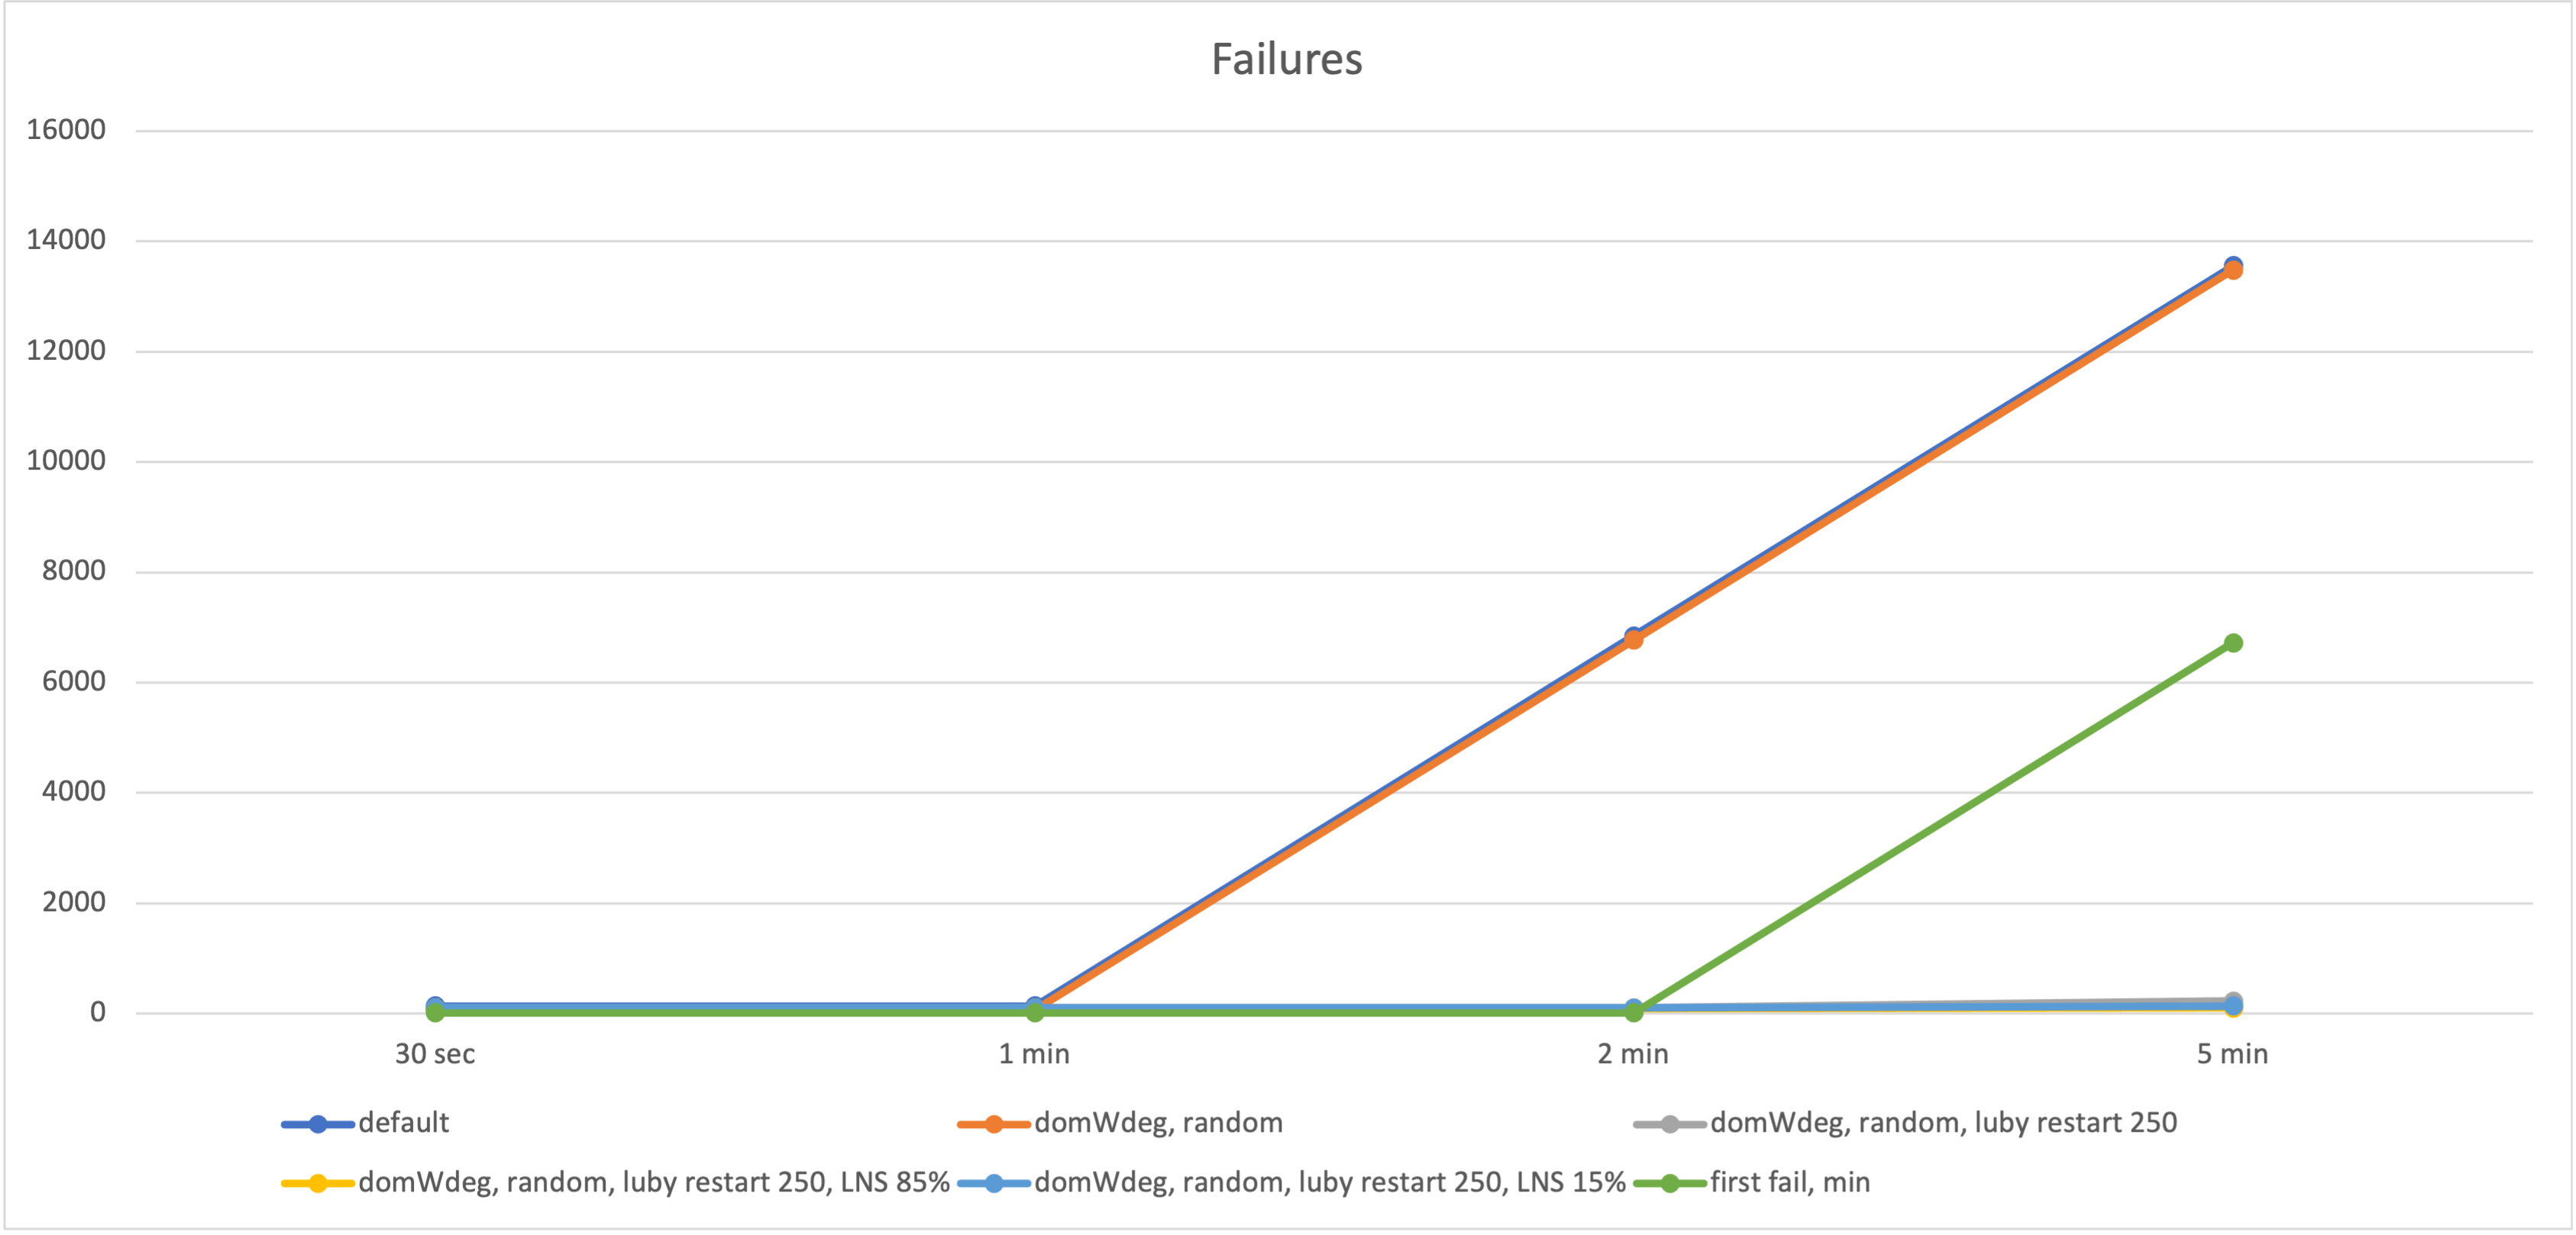
\includegraphics[width=0.8\columnwidth]{../graphs/pr10-failures.png}
    \caption{Failures graph for \textbf{pr10}.}
\end{figure}

{
\renewcommand{\arraystretch}{2}
\begin{longtable}[h]{| c | c | c | c | c |}
    \hline
    \textbf{Objective function} & \multicolumn{3}{c}{Time limit} & \\
    \hline
    \textbf{Search strategy} & \textbf{\textit{30 sec}} & \textbf{\textit{1 min}} & \textbf{\textit{2 min}} & \textbf{\textit{5 min}} \\
    \hline
    \endhead
    default search                                & - & - & 211.167.490 & 210.196.270 \\
    \hline
    domWdeg, random                               & - & - & 195.753.960 & 195.603.480 \\
    \hline
    \textit{domWdeg, random, Luby restart L=250}  & - & - & 208.501.980 & 192.864.620 \\
    \hline
    domWdeg, random, Luby restart L=250, LNS 85\% & - & - & 208.501.980 & 208.467.900 \\
    \hline
    domWdeg, random, Luby restart L=250, LNS 15\% & - & - & 208.501.980 & 206.010.280 \\
    \hline
    first fail, min                               & - & - &         - & 200.835.560 \\
    \hline
\end{longtable}
}
\begin{figure}[H]
    \centering
    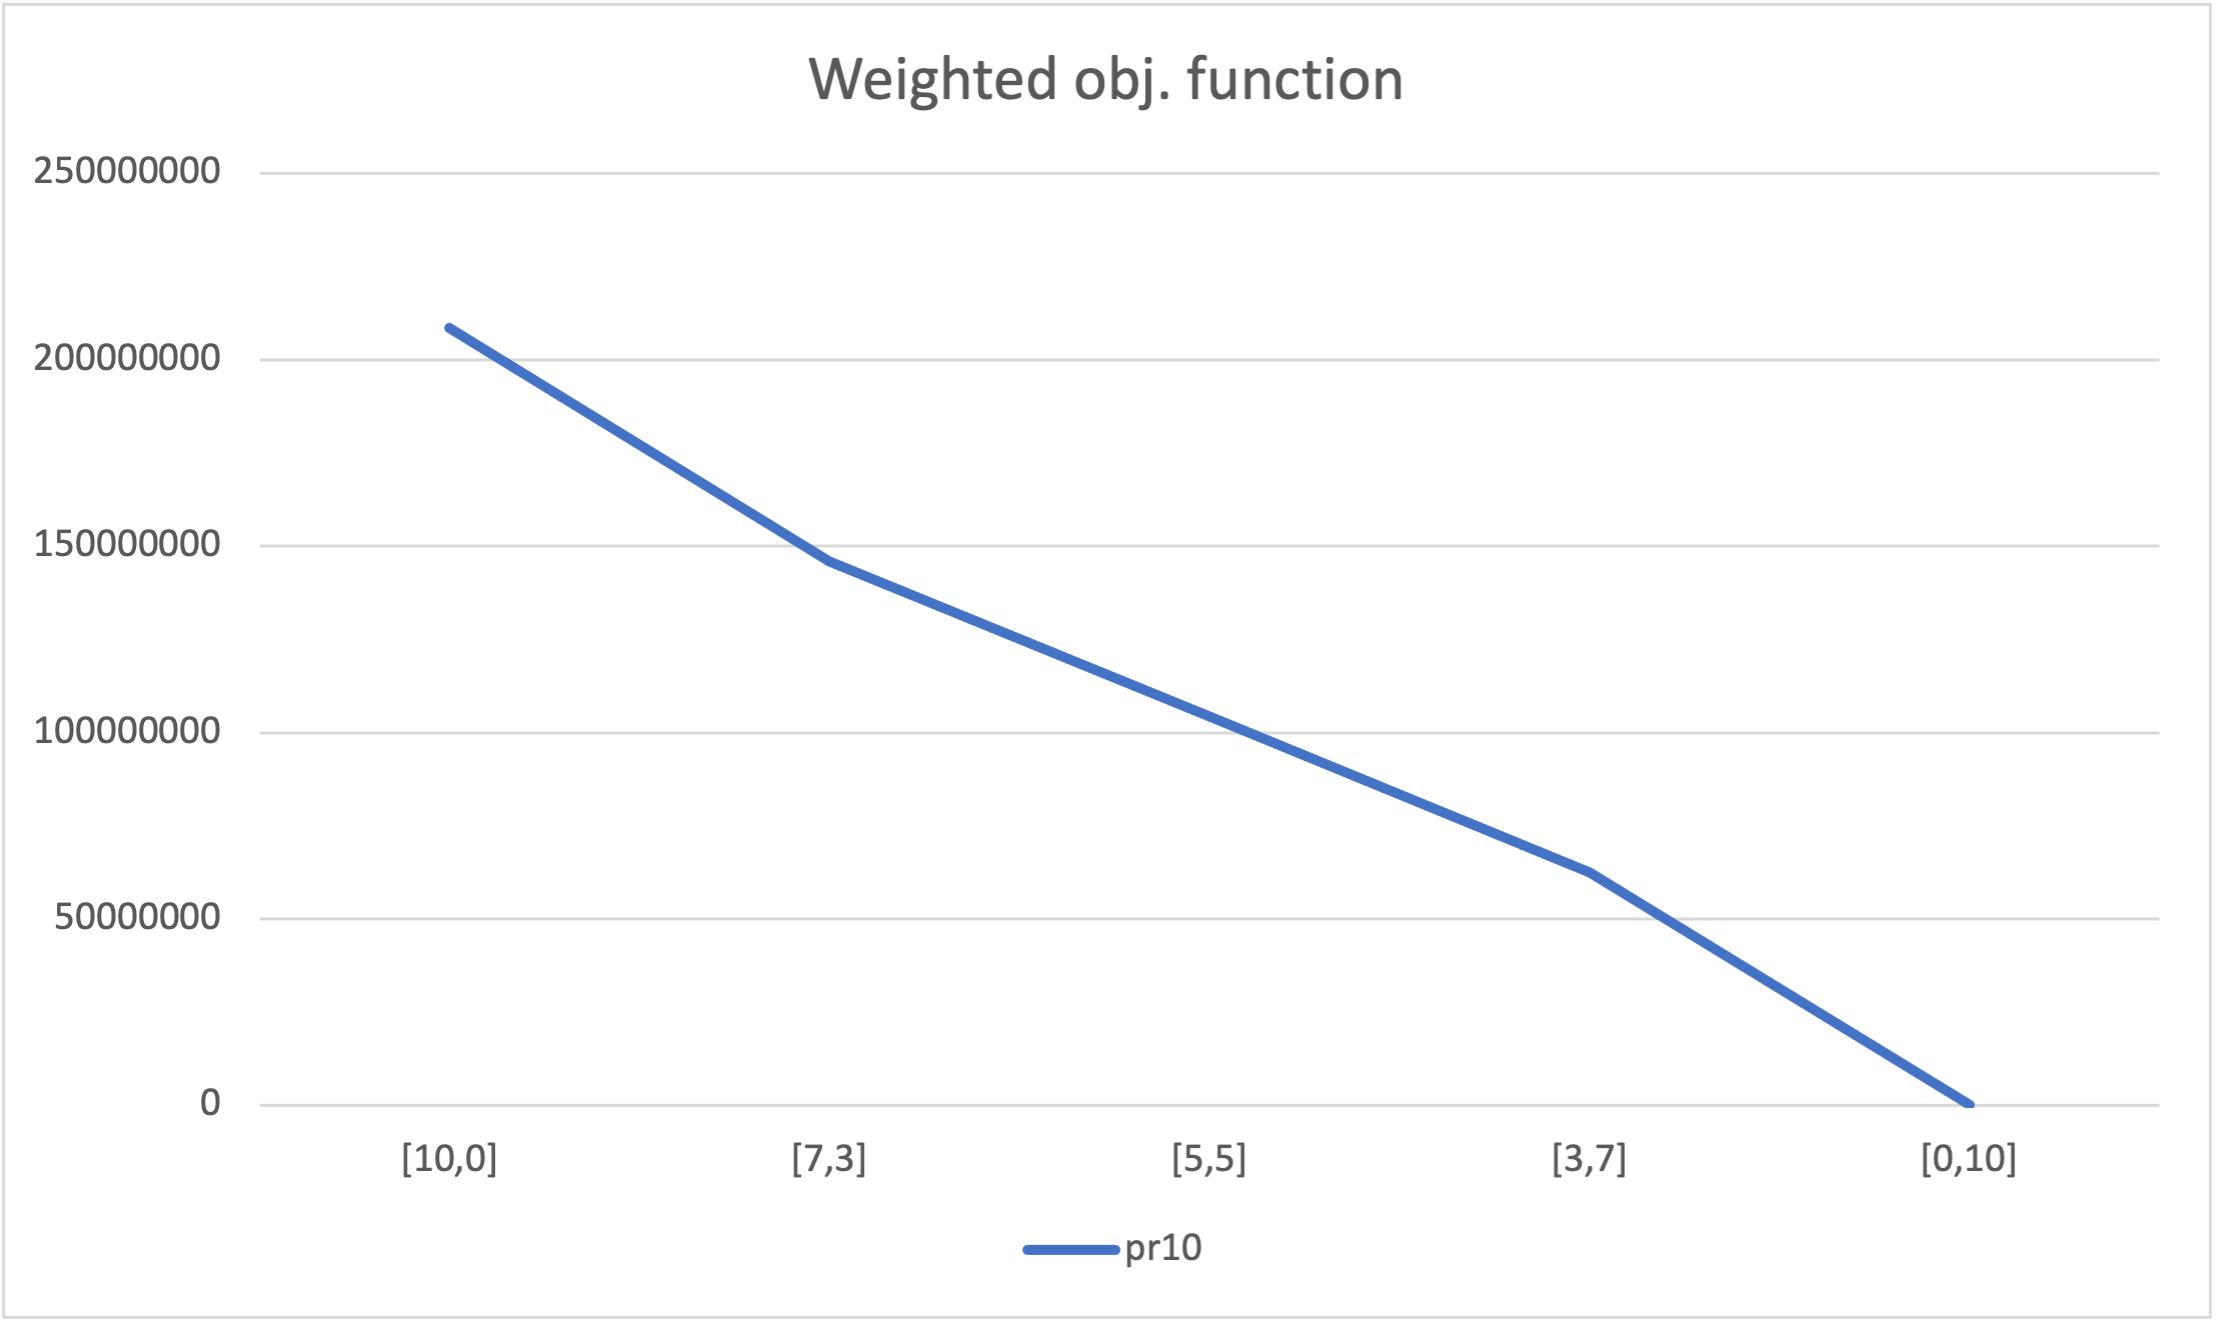
\includegraphics[width=0.8\columnwidth]{../graphs/pr10-wobjf.png}
    \caption{Objective functions graph for \textbf{pr10}.}
\end{figure}

{
\renewcommand{\arraystretch}{2}
\begin{longtable}[h]{| c | c | c | c |}
    \hline
    \textbf{Weights} & \textbf{Objective function} & \textbf{Total distance} & \textbf{Used vehicles} \\
    \hline
    \endhead
    $\alpha = 10, \beta = 0$ & 208.467.900 & 20.846.790 & 20 \\
    \hline
    $\alpha = 7, \beta = 3$  & 145.927.590 & 20.846.790 & 20 \\
    \hline
    $\alpha = 5, \beta = 5$  & 104.234.050 & 20.846.790 & 20 \\
    \hline
    $\alpha = 3, \beta = 7$  &  62.540.510 & 20.846.790 & 20 \\
    \hline
    $\alpha = 0, \beta = 10$ &         200 & 20.850.198 & 20 \\
    \hline
\end{longtable}
}
\begin{figure}[H]
    \centering
    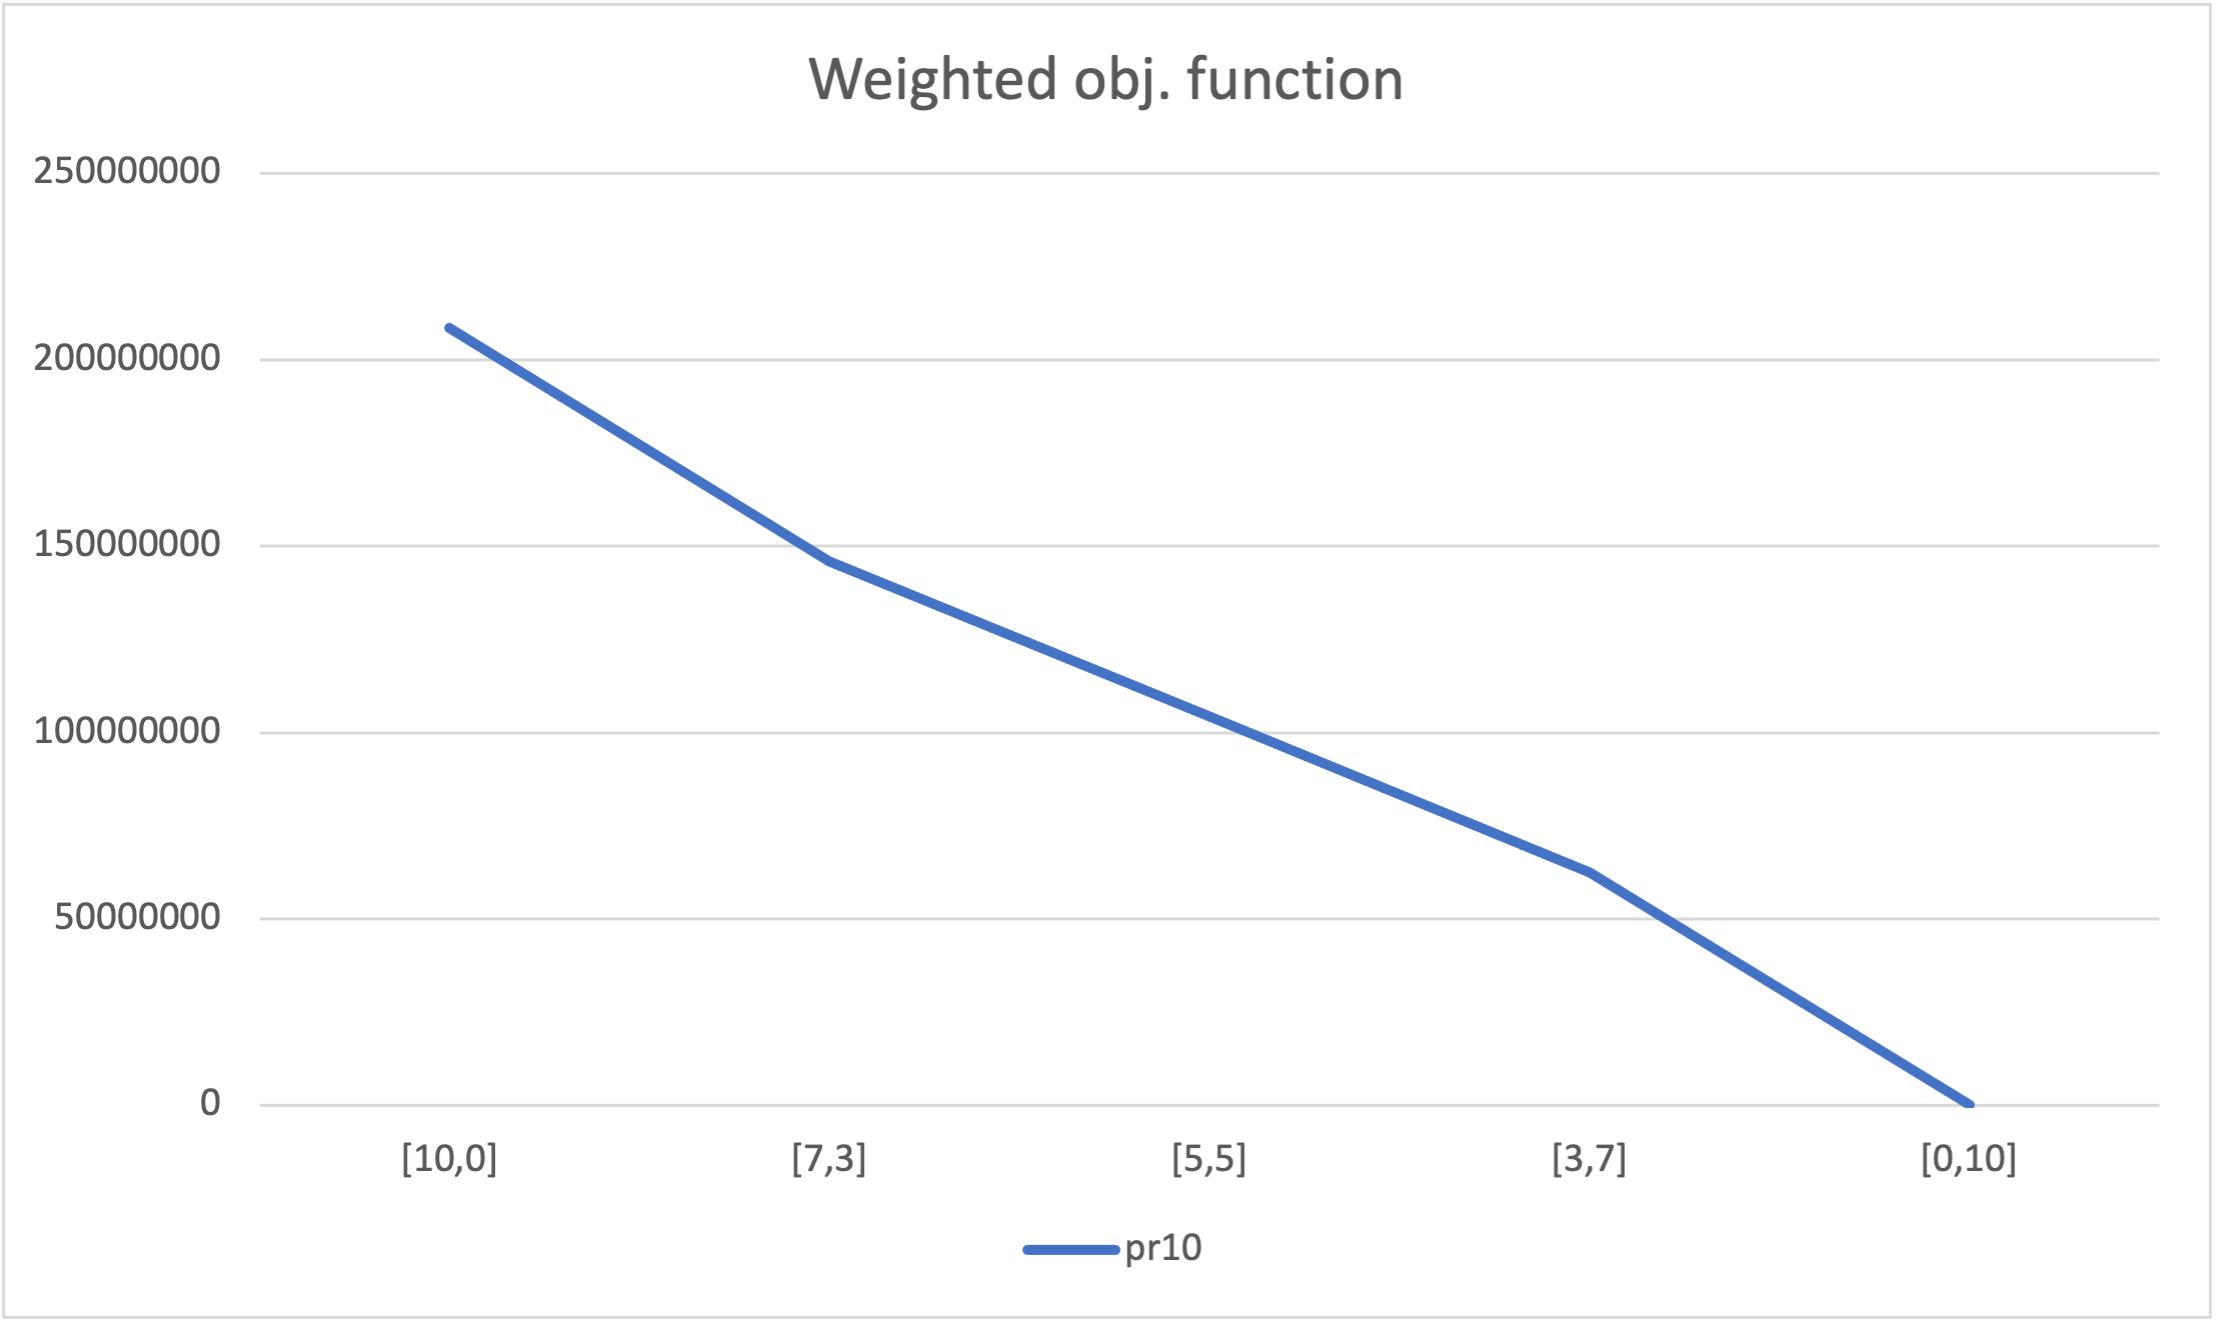
\includegraphics[height=0.25\textheight]{../graphs/pr10-wobjf.png}
    \caption{Weighted objective functions graph for \textbf{pr10}.}
\end{figure}

\begin{figure}[H]
    \centering
    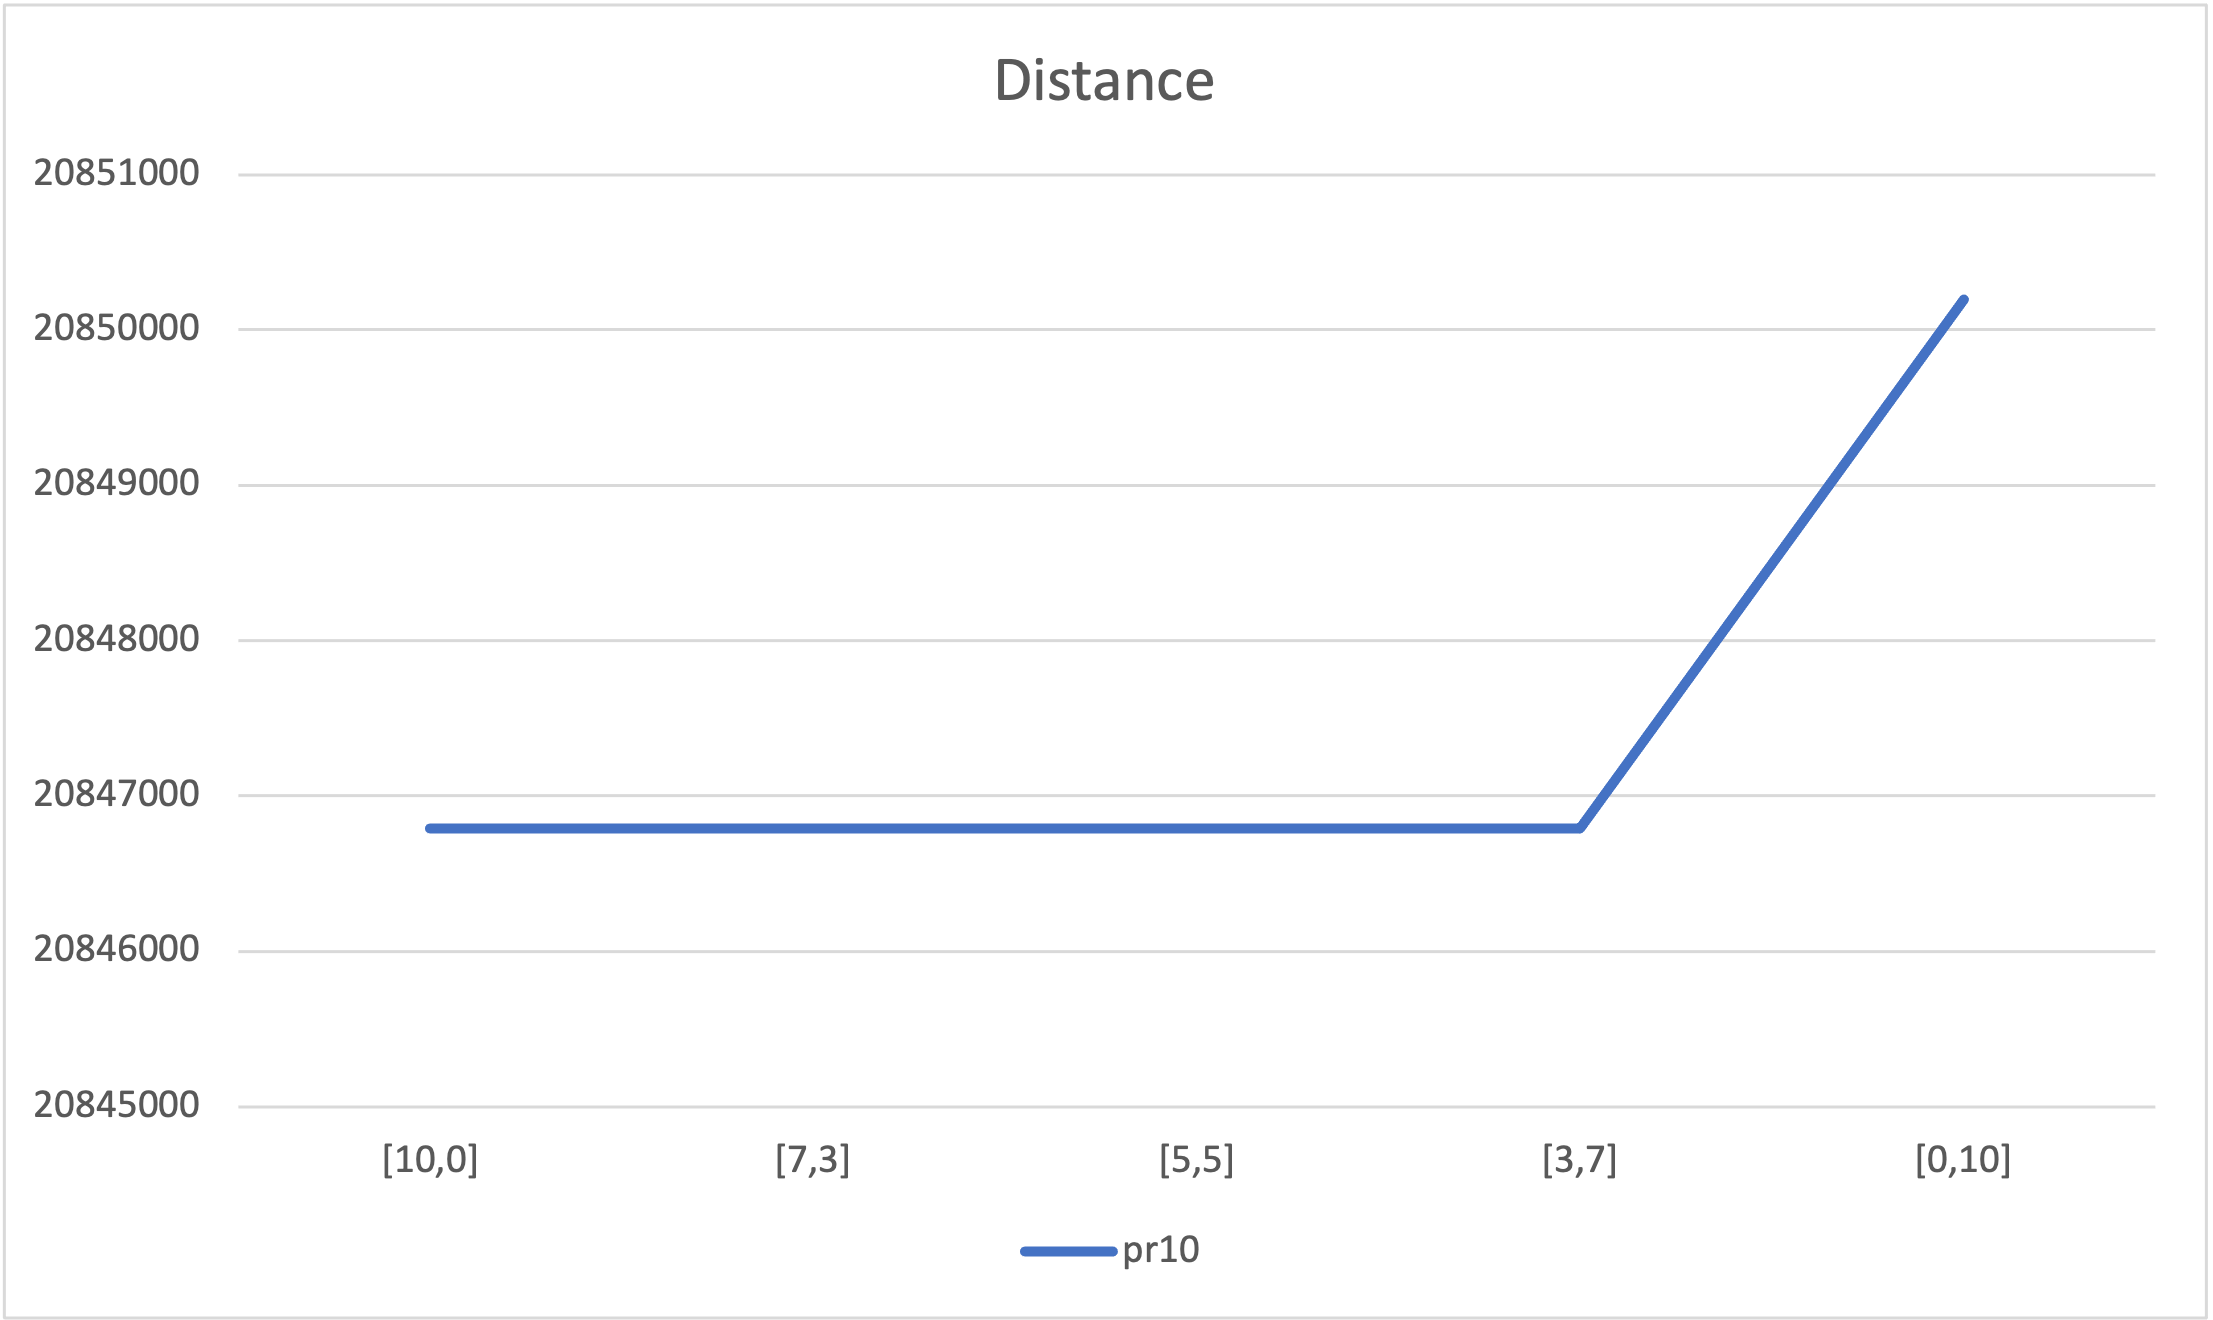
\includegraphics[height=0.25\textheight]{../graphs/pr10-distance.png}
    \caption{Distances graph for \textbf{pr10}.}
\end{figure}

\begin{figure}[H]
    \centering
    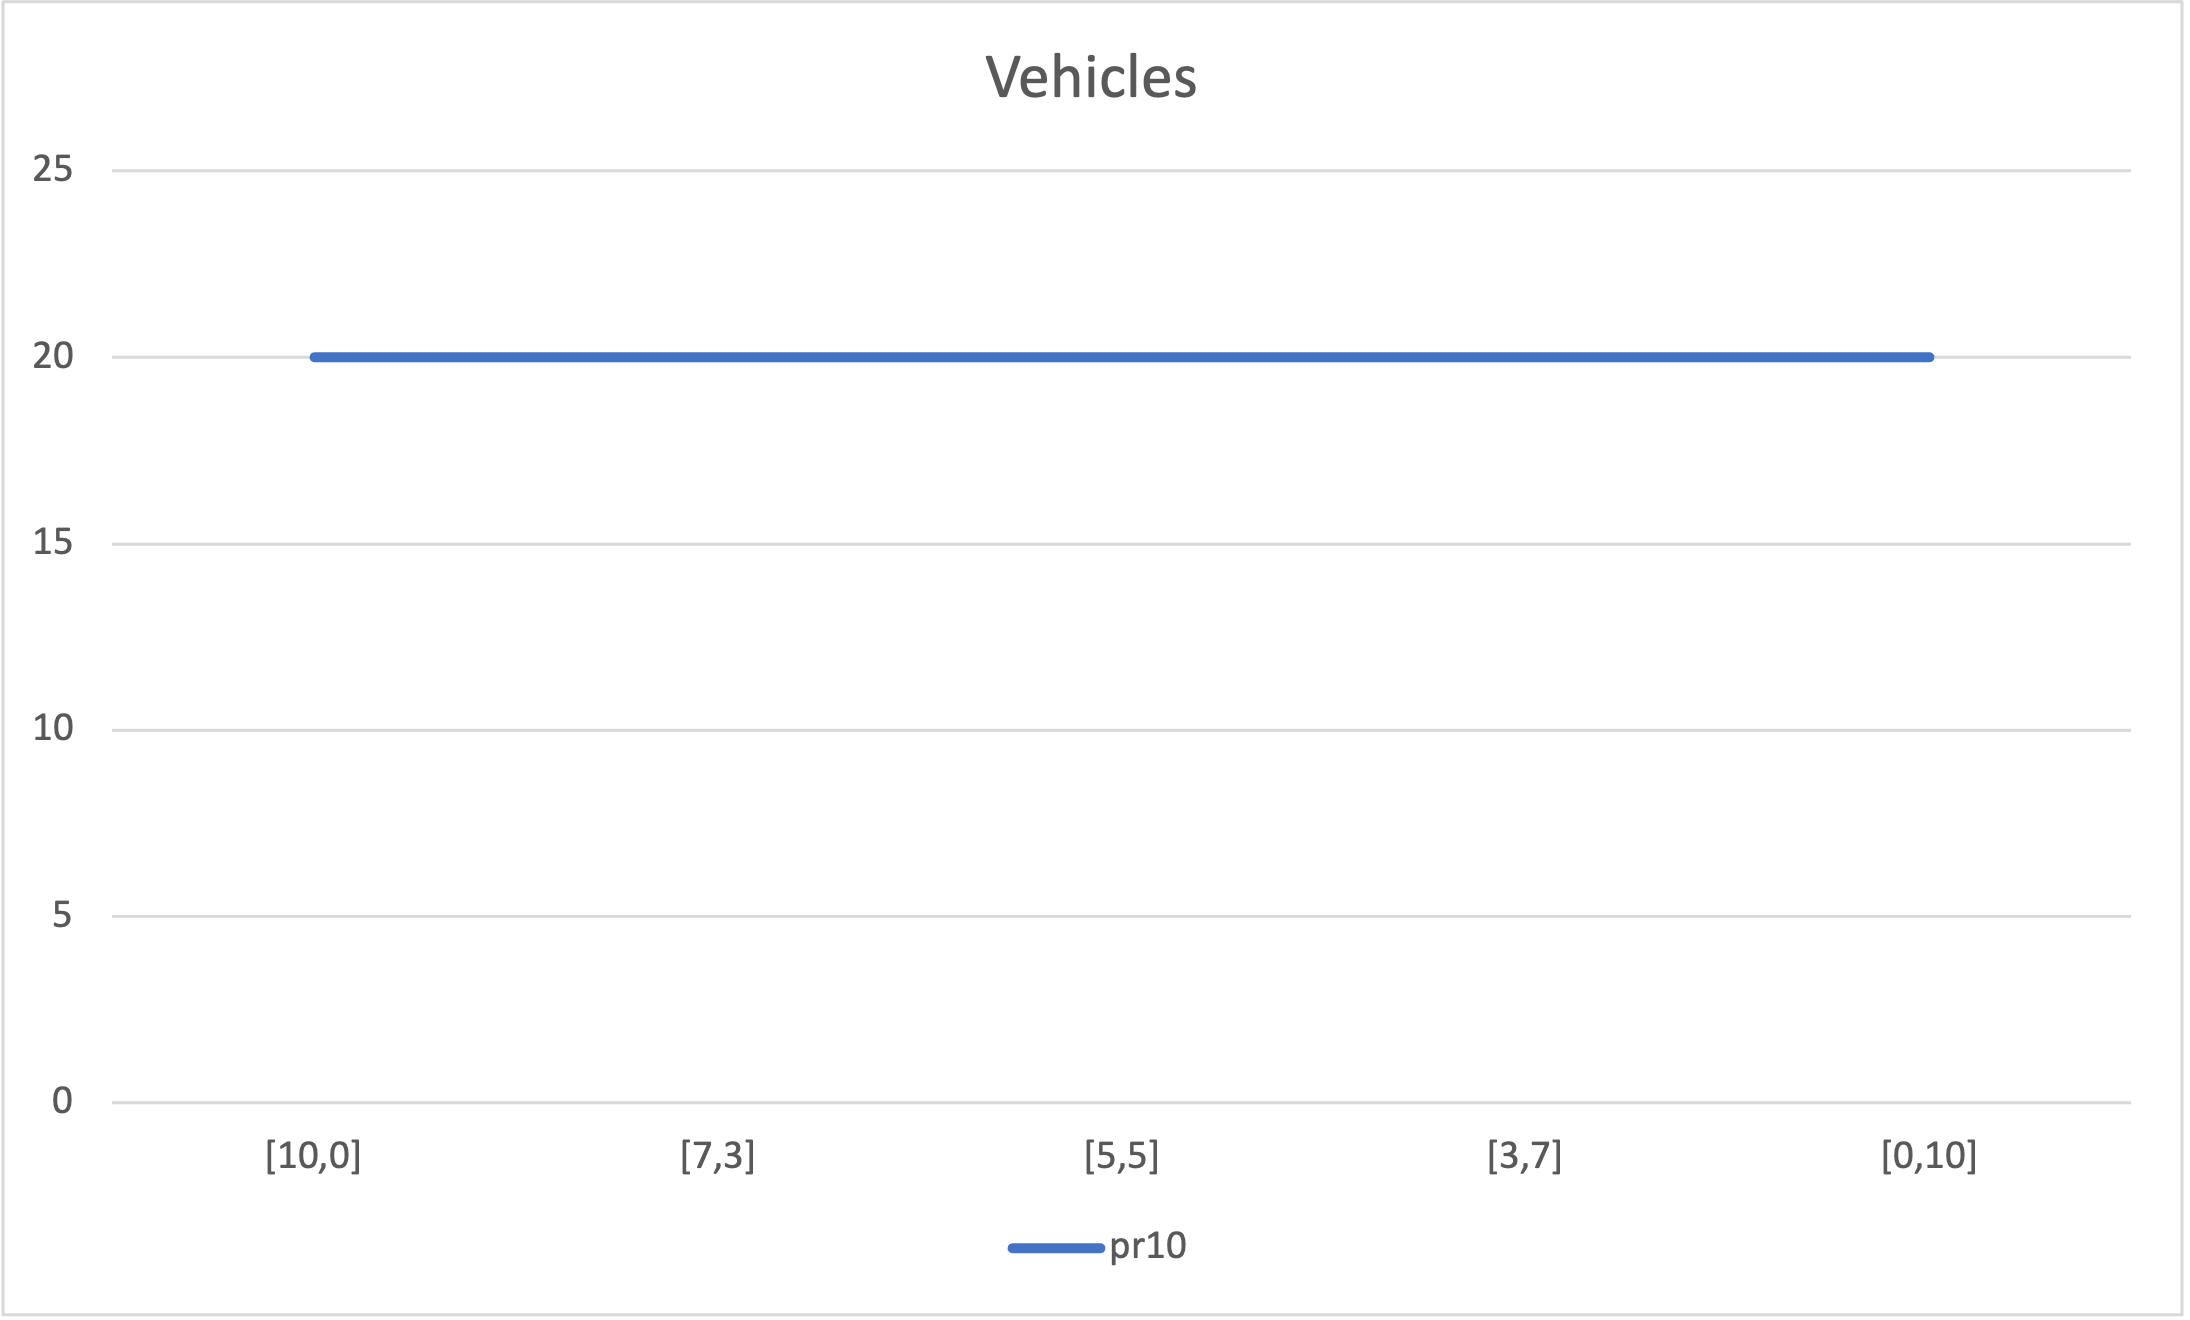
\includegraphics[height=0.25\textheight]{../graphs/pr10-vehicles.png}
    \caption{Vehicles used graph for \textbf{pr10}.}
\end{figure}

\newpage